%% This is the Chapter 4

%\begin{hyphenrules}{nohyphenation}
\chapter{PREDICTING RATES OF EVOLUTION FOR ONE TRAIT USING A CONTINUOUS GRADIENT OF ANOTHER TRAIT}
%\end{hyphenrules}

\section{Abstract}

To be done.

\section{Introduction}

There is a striking degree of phenotypic diversity among groups of species across the tree of life. Many are the factors that influence the tempo and mode of phenotypic evolution \citep[e.g.,][]{adams_are_2009, cooper_what_2009, hipsley_morphological_2014}. Furthermore, shifts in the pace of trait evolution, which can disconnect phenotypic disparity from clade age, are common throughout the history of several groups \citep{Eastman_2011, benson_rates_2013, mahler_exceptional_2013, Rabosky_2013, slater_phylogenetic_2013, rabosky_analysis_2014, Uyeda_BayOU}. These shifts are often associated with important events on the evolutionary history of lineages, such as mass extinctions \citep{slater_phylogenetic_2013}, the evolution of a new function for an existent trait \citep{benson_rates_2013, dececchi_body_2013} or even changes in the structure of evolutionary correlation among traits affecting the ability of lineages to explore novel regions of the morphospace \citep{revell_phylogenetic_2009, caetano_sysbio_2017}.

Changes in the tempo and mode of evolution of lineages are often interpreted as instantaneous shifts in the history of the group. On a phylogenetic context, discrete evolutionary events are mapped to specific locations on branches or nodes of the tree following ancestral reconstruction analyses \citep{schluter_likelihood_1997, pagel_maximum_1999, huelsenbeck_stochastic_2003}. These positions then divide the phylogenetic history of the group into different regimes defined by the presence or absence of the events under study \citep{butler_phylogenetic_2004, omeara_testing_2006, revell_phylogenetic_2009, Eastman_2011, caetano_sysbio_2017}. This framework is the most used to study macroevolutionary patterns of trait evolution using available phylogenetic comparative methods (PCMs) and is grounded in the concept of `key innovations' \citep{simpson_1953, heard_key_1995} as the driver of trends in phenotypic evolution. Interestingly, most macroevolutionary studies are focused on the influence of rare events on the history of the groups even though the reduced number of observations is prone to bias results due to the problem of phylogenetic pseudo-replication \citep{maddison_unsolved_2015}. Whether such focus is a result of an inordinate fondness for unique, and often extraordinary, events across the tree of life or a paradigm associated to the history of comparative studies is hard to understand.

On the other hand, not all traits acting as important driving forces of phenotypic evolution among lineages are essentially discrete. Important factors such as climate \citep{hunt_simple_2015, clavel_accelerated_2017}, degree of species interactions \citep{galetti_functional_2013, thompson_diversification_2013}, range size \citep{Diniz_range_1998, pigot_speciation_2012}, and habitat specialization \citep{bonetti_evolution_2014, hardy_specialization_2014} are inherently continuous. Continuous traits are not naturally interpreted on a phylogenetic context by the use of discrete transitions or regimes. Furthermore, while discrete `key innovations' are commonly associated with shifts in the tempo and mode of phenotypic evolution \citep[e.g.,][]{revell_phylogenetic_2009, claverie_modularity_2011, benson_rates_2013, dececchi_body_2013, maddison_unsolved_2015}, continuous factors are often addressed as predictors on regression models that use phylogenetic information only as a means to address the lack of independence among species traits \citep{felsenstein_1985, grafen_phylogenetic_1989, blomberg_independent_2012}. However, continuous traits can also have important impacts on the tempo and mode of phenotypic evolution and, similar to regimes mapped for a discrete trait, the gradient of a continuous variable across the branches of the phylogenetic tree could be used as a predictor for the dynamics of phenotypic evolution.

Most phylogenetic comparative models of trait evolution focus on the macroevolutionary patterns of single traits \citep{butler_phylogenetic_2004, omeara_testing_2006, Eastman_2011, rabosky_analysis_2014, Uyeda_BayOU}. Evolutionary rates for traits are estimated based on species mean values, the distribution of branch lengths, and the topology of the tree whereas rate shifts are estimated in function of the evolutionary variance for the trait estimated on different regions of the tree \citep{omeara_testing_2006, Eastman_2011}. Some methods allow rate regimes to be mapped \textit{a priori} to the phylogeny following another discrete variable \citep{butler_phylogenetic_2004, omeara_testing_2006} while others automatically find the location of shifts \citep{Eastman_2011, rabosky_analysis_2014, Uyeda_BayOU}. More recently, models have incorporated continuous varying rates of trait evolution across the branches of the tree, but such rates vary independently of any predictor variable \citep{rabosky_analysis_2014}. In the case that two or more continuous traits are incorporated into the analysis, models use variance-covariance matrices to estimate both the rate of evolution for each trait and their evolutionary covariance \citep{revell_phylogenetic_2009, bartoszek_phylogenetic_2012, Clavel_mvmorph, caetano_sysbio_2017}. However, up to date, no comparative model is able to estimate rates of trait evolution for a continuous trait as predicted by another continuous variable mapped to the same tree.

We present a novel framework that uses mathematical functions to describe the dynamics of rates of evolution of a continuous trait with respect to the values of a predictor variable mapped to the phylogenetic tree. For this we model rate variation alongside the branches of the phylogeny using a semi-continuous approach. At each branch, rates of trait evolution are predicted using some continuous mathematical function mapping to the values of the predictor variable. We show that the new approach estimates meaningful patterns of rate variation throughout the tree using different mathematical functions and provide a approach to test the predictive power of gradients to explain rates of trait evolution across phylogenetic trees.

\section{Methods}

\subsection{Description of the model}
% The root for the Q matrix estimate using fitDiscrete might be different than when making stochastic maps with make.simmap. By default make.simmap will set the prior for the root as flat. I do not know what is the default behavior for fitDiscrete, however this is an important thing to be aware of. If the root behviour is very distinct, it might be a good idea to change something for them to be more compatible. One thing is that we have information about the root of the model since the BM model will have root close to the mean of the data.

Here we use continuous mathematical functions to model the rates of evolution of a trait (i.e., the response trait) under a Brownian-motion model (BM) with respect to the values of another trait (i.e., the predictor trait). The model aims to study the association between the macro-evolutionary patterns of one trait evolving on a phylogenetic tree and the rates of evolution of another trait on the same tree. Figure \ref{fig:model_example} shows the fundamental concepts of the model. The predictor and response traits are continuous traits for the same set of species. The linear function represented by the line on Figure \ref{fig:model_example} describes the variation of evolutionary rates for the response trait ($\sigma^{2}_{response}$) in function of the trait values of the predictor trait. The difference between the present model and other phylogenetic comparative models of trait evolution with varying rates, such as AUTEUR \citep{Eastman_2011}, BAMM \citep{rabosky_analysis_2014}, and bayOU \citep{Uyeda_BayOU}, is that these methods estimate rates of trait evolution informed only by the distribution of trait values and the phylogenetic tree. In contrast, here we introduce the use of a second trait to inform the variation of rates of evolution across the branches of the tree.

The model can be sub-divided into two components; ancestral values for the predictor trait are mapped to the branches of the phylogenetic tree and evolutionary rate regimes for the response trait are assigned to the phylogeny in function of the map of ancestral predictor trait values. First we divide the predictor trait into $\mathit{k}$ ordered categories defined by $\mathit{k}$ - 1 equidistant breakpoints across the range of the predictor trait values. Then we estimate the evolutionary rate transitions among the $\mathit{k}$ categories using a Markov process \citep{pagel_detecting_1994} that restricts transition rates to happen only between neighbouring states. For example, a transition from $\mathit{k_{i}}$ to a larger trait value category $\mathit{k_{i+3}}$ need to be preceded by transitions to and from the intermediary categories $\mathit{k_{i+1}}$ and $\mathit{k_{i+2}}$. The number of categories reflects how fine-grained is the model with respect to the macro-evolutionary patterns of the (continuously distributed) predictor trait; larger $\mathit{k}$ produce a more fine detailed model whereas smaller $\mathit{k}$ yield a more coarse model \citep{boucher_inferring_2016}.
% The comment made in this paragraph calls for a sensitivity test regarding the number of categories used to describe the predictor trait. This is an essential result and should be included in the chapter.

The transition rates between the $\mathit{k}$ categories of the predictor trait can be estimated using a meristic Markov model (MKn) with a single homogeneous rate or multiple rates. Homogeneous rate can be described by constraining all transition rates between neighbouring categories to be equal whereas more complex evolutionary patterns can be described by allowing transition rates to and from each category to vary. Of course, one can compare and choose the model that best describes the evolutionary history of the predictor trait across the branches of the phylogenetic tree. As the number of categories ($\mathit{k}$) increases the single rate Mkn model becomes equivalent to a single rate Brownian-motion (BM) model whereas the unconstrained Mkn model spans trait evolution models with heterogeneous rates such as multiple rate BM \citep{omeara_testing_2006}, BM with a directional trend \citep{hunt_fitting_2006} and Ornstein–Uhlenbeck \citep[OU --][]{butler_phylogenetic_2004} \citep{boucher_inferring_2016}. However, the Mkn model, as used here, fits a single transition matrix to the whole phylogenetic tree and, as a result, can only be equivalent to time-dependent models, such as the accelerated/decelerated \citep[ACDC --][]{blomberg_testing_2003, uyeda_comparative_2015} and early burst \citep[EB --][]{harmon_early_2010}, if the predictor map shows a time-dependent structure.
% Although the free model spans the 'BM with a trend', because of the way the estimation works and because the categories are defined using the tip data, it is very unlikely (maybe impossible) for the 'BM with a trend' model to be one of the estimated models.

In order to map ancestral values of the predictor trait to the branches of the phylogenetic tree we generate multiple stochastic histories for the trait categories using the estimated Mkn transition matrix \citep{huelsenbeck_stochastic_2003}. Each of these maps associate the branches of the phylogeny with the $\mathit{k}$ categories for the ancestral values of the predictor trait. Then we use a mathematical function (see Figures \ref{fig:bio_functions} and \ref{fig:model_example}) to map these predictor trait regimes to evolutionary rate regimes for the response trait and compute the likelihood of a multiple rates Brownian-motion model \citep{omeara_testing_2006} with the response trait as the tip data.

\subsection{Mathematical functions and model choice}
% Talk a little that we are using MLE estimation, but that MCMC or even RJMCMC can be implemented. This is more suitable to the Discussion section.

Virtually any mathematical function can be used to map values of the predictor trait categories to evolutionary rate regimes of the response trait. Different functions can be fit to the data using maximum likelihood (ML) and compared using standard model choice approaches such as Likelihood-ratio tests (LRT) for nested or the Akaike information criterion (AIC) for non-nested models \citep{burnham_model_2003}. Using model choice criteria that penalizes for the number of parameters \citep[such as AIC --][]{burnham_model_2003} is desirable, since distinct functions of varying complexity can produce identical maps. Some mathematical functions are commonly applied across a series of biological disciplines and are likely to be erected as \textit{a priori} hypotheses for the macro-evolutionary association between a plethora of traits. Figure \ref{fig:bio_functions} shows a collection of functions that describe patterns commonly observed in biological data, especially in studies of trait evolution using phylogenetic trees.

One of the advantages of our approach is that the number of parameters varies with respect to the chosen mathematical function rather than the number of categories used to describe the predictor trait (see Figure \ref{fig:bio_functions}). This is a result of maximizing the likelihood of the data with respect to the parameters of the mathematical function rather than to the rate regimes directly. Thus, we can use a large number of rate regimes in order to model a trait with  (semi-)continuously varying rates of evolution across the phylogeny without increasing the number of parameters of the model. This aspect of the model is similar to the strategy implemented in BAMM \citep{rabosky_2014}, which uses an exponential function to describe the continuous decrease or increase of rates of trait evolution through time.

\subsection{Model implementation}

We implemented the model as a R package named \texttt{`phylofx'}. The package offers a simple interface to fit continuous mathematical functions to model the variation of evolutionary rates of a response trait in function of a predictor trait across the branches of a phylogenetic tree. All mathematical functions showed on Figure \ref{fig:bio_functions} are available in the package and can be chosen from a simple menu. The package also have options for users to define their own mathematical functions.

\subsection{Performance simulations}
% One aspect of the model that was not explored by the simulations is the possible case in which rates of evolution are heterogenic over the phylogeny but that the shifts have no relation with any other trait. What happen with the model selection? It is likely that a more complex model will be selected in this case. Maybe it is a good idea to use another model when doing this tests. Maybe we can test the AIC scores against a aeuteur model? The aeuteur model will accomodate heterogenic rates of trait evolution without relating it to any other trait. This is a good thing to think about and is similar to the issue addressed by Beaulieu and O'Meara.

To check the performance of the method we will focus in three very common, but distinct, nested models: a constant relationship, with homogeneous evolutionary rates ($\sigma^{2}$=0.5); a step function, with two distinct rates separated by an instantaneous transition step ($\sigma^{2}_{left}$=1, $\sigma^{2}_{right}$=0.5, break point=mean of predictor trait); and a linear function, with a continuous relationship between the predictor and the response traits (see Figure \ref{fig:bio_functions}). For the linear function we defined $\beta_{1}$=0.5, the set of predictor trait values at the tip as $X$, and computed the intercept such that:

\begin{equation}
\beta_{0} = \beta_{1} \ min X - 0.1
\end{equation}

We generated a phylogenetic tree with 200 species using a pure-birth model (tree height=1). Then we simulated a predictor trait following a single rate BM model ($\sigma^{2}$=0.5) and divided it into 10 trait categories mapped to the branches of the tree. We will refer to the result of this simulation as the true mapped tree. We used the true mapped tree to assign evolutionary rate regimes to the branches following one of the mathematical functions described above and simulated the response trait under a multi-rate BM model. We repeated this process in order to produce 100 datasets for each of the three mathematical functions used in the simulations tests.

In order to fit the models to the generated data, we estimated a meristic Mkn transition matrix for the predictor trait with $\mathit{k}$=5 and equal transition rates. We produced 10 stochastic mapping histories based on this transition matrix and performed a maximum likelihood estimate for each of the mathematical functions under each of the stochastic mapping histories. We chose the best model by comparing the mean pairwise AIC values across all stochastic maps with threshold equal to 4 $\Delta$AIC units \citep{burnham_model_2003}. We repeated model fit and model test for each of the 300 simulated datasets. We computed error rates as the frequency in which the model used to generate the data was not selected as the best model.

Preliminary tests showed that it is often difficult to find the global maximum likelihood for the parameters of the model using minimization algorithms. Thus, we applied three distinct strategies to generate the starting point for the searches. First we generated starting points by drawing from a flat distribution with a large range of parameter values (from -400 to 400). Starting points generated using this approach are unlikely to be close to the global maximum but provide a wide sample of the parameter space. We refer to this approach as `wide'. Second we used a more informed strategy by optimizing the parameters of the mathematical functions to produce evolutionary rates equal to $\sigma^{2}$ estimated for a homogeneous BM model with the response trait as the tip data. Then we defined a narrow range of parameter values around the best fit (by adding -10 and 10) and used this distribution to draw starting points. This starting point strategy, which we refer as `narrow', makes sure that starting parameter values for the functions yield evolutionary rates that are congruent with the observed data and avoid possible problems resulting from starting at a flat region of the likelihood surface. Finally, we applied the most informative strategy by setting the starting point of the ML searches as the true parameter value for the models. When estimating a model different from the one that generated the data we set the parameters of the mathematical function as to minimize the distance relative to the evolutionary rates predicted by the true model for each trait category. We defined this search strategy as `fixed'. We compare and discuss results among the different search strategies.

%\subsection{Sensitivity to trait categorization}
% In a subsequent test I might be able to make a more comprehensible thing by increasing the number of categories of the true model or even making a full continuous simulation.

%Our model associates the evolutionary rates of a continuous response trait to the trait values of a continuous predictor trait by transforming the data into ordered categories. On one hand, if the number of trait categories is large enough the trait evolution model converges with continuous models, such as Brownian-motion. On the other hand, this raises concerns about the adequacy of the model and parameter estimates when one applies only a small number of trait categories.

%In order to test the sensitivity of the model to the number of trait categories ($\mathit{k}$), we simulated data following the same approach described above for performance simulations. However, we increased the number of trait categories to 15 and simulated datasets only with the linear function. We estimated parameter values for the linear model and performed model test using $\mathit{k}$ equal to 15, 10, and 5. Then we computed the distance between estimated parameter values to the true parameter values and the frequency that the generating model was chosen as the best model.

\subsection{Likelihood surface for the linear function}

Results from simulations showed that the linear model estimated with starting points draw from a wide range of the parameter space (the `wide' strategy) often have worse fit than estimates with starting points informed by the data (the `narrow' strategy). To investigate whether this pattern is associated with the shape of the likelihood surface rather than a systematic bias due to the implementation of a restricted pool of starting points when using the `narrow' strategy we computed summary statistics from the results of maximum likelihood searches based on the simulated data.

First we calculated the number of times that the multiple independent searches for the same data reached the maximum likelihood score among all the searches, we defined this quantity as `hits'. To compute the number of `hits' we aggregated the maximum likelihood score returned by each of the independent searches. Then we counted the number of searches for which the $\Delta$log-likelihood with respect to the maximum log-likelihood among all searches was less than the 0.0001 threshold. A large number of `hits' indicates that multiple searches starting from different points in the parameter space converged towards the same likelihood score and, therefore, the same combination of parameter values. Such result support the hypothesis that this point is the global maximum log-likelihood for the model. Following, we investigated whether there is an association between the number of `hits' and how close is the model estimate to the true model that generated the data. For this we only used results based on the same models that generated the data.

\section{Results}

\subsection{Performance simulations}

First we computed the proportion of times that each of the generating models was recovered by model selection using the Akaike information criterion (AIC) while integrating the uncertainty associated with the use of stochastic mapped histories and comparing different approaches used to define the starting points for the maximum likelihood searches. Table \ref{tab:best_aic_sims} shows the number of times among all 100 simulated datasets that each model had the best AIC score, computed as the mean pairwise AIC over stochastic mapped histories. Then we used $\Delta$AIC scores, also based on the pairwise AIC across stochastic mapped histories, to record support for (Table \ref{tab:support_true_model}) and against (Table \ref{tab:reject_true_model}) the model that generated the data using a threshold of 4 $\Delta$AIC units. For each simulation replicate and starting point strategy we plotted the distance between $\sigma^{2}$ values for the predictor trait categories estimated under the models and the true value for the simulation (Figures \ref{fig:chart_const}, \ref{fig:chart_linear} and \ref{fig:chart_step}). Below we describe results when data are simulated with the constant, linear, and step functions.

The majority of replicates, independent of search strategy, recovered the true model as the model with best AIC scores when data was generated under a constant evolutionary rate throughout the tree (Table \ref{tab:best_aic_sims}). However, for most cases, there is a lack of support in favor (Table \ref{tab:support_true_model}) or against (Table \ref{tab:reject_true_model}) the constant model when compared with alternative models. These results suggest that $\Delta$AIC cannot substantiate any difference between models when data is simulated under a constant rate of evolution. Indeed, the distance between rates estimated for each model and the true rates is comparable among most of the replicates, starting point strategies, and models (Figure \ref{fig:chart_const}). Only the linear function estimated using the `wide' starting point strategy can be rejected as a good model to explain the data when contrasted with the true model. Figure \ref{fig:chart_const} (top row, middle column) shows that rates estimated under this model are much larger than reasonable values given the tree and the trait data, which suggests that the estimator failed to find the global maximum for the likelihood of the model.

Data generated under the linear function, where rates of evolution of the response trait show a positive correlation with predictor trait values, show results with the true model having the highest AIC on the majority of simulation replicates for both the `narrow' and `fixed' starting point approaches (Table \ref{tab:best_aic_sims}). However, this result changes in the case of the `wide' distribution of starting points, because the step function shows the best AIC scores even though the data was simulated under a linear function. When we compute the support for the model that generated the data both under the `narrow' and `fixed' starting points, we see that there is support for the linear model against the constant model on the majority of replicates and about half of the replicates show support in favor of the linear model when compared with the step model (Table \ref{tab:support_true_model}). On the other hand, when using the `wide' starting point distribution, $\Delta$AIC scores point to both alternative models as better models than the true model that generated the data (Table \ref{tab:reject_true_model}). Parameter estimates for these models show that results from the linear model under the `wide' starting point strategy produce overly large evolutionary rates compared to competing models (Figure \ref{fig:chart_linear} - top row, middle column), which is likely the reason for the poor fit to the data. Using either the `narrow' and `fixed' starting point produce better parameter estimates for the linear function (Figure \ref{fig:chart_linear} - middle and bottom rows) that reflect as more support for the true model based on $\Delta$AIC scores (Table \ref{tab:support_true_model}).

The step model is the most parameter-rich among the tested models, with three parameters (see Figure \ref{fig:bio_functions}). When data was simulated under this model, only results from the `wide' starting point distribution show the true model as the model most frequently with the highest AIC scores (Table \ref{tab:best_aic_sims}). Under the other starting point strategies the step model is as frequent the best AIC scoring model as the linear model (Table \ref{tab:best_aic_sims}). This pattern is also present in the results of the support for the step model over alternative models. When using the `wide' starting point distribution the step model is favored over the linear model in the majority of replicates whereas there is no difference between these models in the majority of replicates when using the other starting point approaches (Tables \ref{tab:support_true_model} and \ref{tab:reject_true_model}). Parameter estimates for the linear function under the `wide' starting point distribution show the same pattern as in the previous results: rates are too fast and too distant from the parameters that generated the data (Figure \ref{fig:chart_step} - top row, middle column). On the other cases the rates estimates for the linear and the step models show good fit to the data.

\subsection{Likelihood surface for the linear function}

The maximum likelihood estimate (MLE) for the parameters of the different mathematical functions show a trend that the `wide' approach to sample starting points often result in worse fit than the other starting point strategies (see Figures \ref{fig:chart_const}, \ref{fig:chart_linear}, and \ref{fig:chart_step}). When we compute the number of `hits' among all replicates, each with 500 independent searches, for the `wide' and `narrow' starting point distributions we can see that the same trend is reflected in how often independent searches return the same maximum likelihood point. Figure \ref{fig:hist_hits} (middle row) shows the distribution of frequencies of number of `hits' for the linear function using the `wide' and `narrow' starting schemes. When using the `wide' starting point distribution, almost all replicates returned only a single `hit' whereas the frequency of 2 or more `hits' increase significantly under the `narrow' search strategy. Interestingly, the effect of the `wide' distribution of starting point on the number of `hits' is not so pronounced with the other models in the set (Figure \ref{fig:hist_hits}).

The association between a small number of `hits' and poor parameter estimates for the model is made clear by the results shown in Figure \ref{fig:pardist}. The mean absolute distance between the parameter estimates and the true value for the model is larger when the search result returned a single `hit' than when 2 or more `hits' occur. Furthermore, the variance of this distance is much larger when the search resulted in a single `hit', meaning that one is likely to get a maximum likelihood estimate far from the parameter values that generated the data. Surprisingly, there is no gradual improvement in estimates with the number of `hits', searches with 2 or more `hits' show similar mean and variance of the distance between estimated and true parameter values for the model (Figure \ref{fig:pardist}).

\section{Discussion}

The models described herein test for an association between a continuous trait and the evolutionary rates of a second trait evolving on the same phylogenetic tree. We tested the performance of three nested models using simulated datasets: the constant, linear and step functions. However, the same analysis framework used here can be easily extended to any mathematical function, nested or non-nested, that relates the values of a predictor trait to rates of evolution of a response trait under a Brownian-motion model. For instance, the R package \texttt{phylofx} provides six functions that can be easily implemented (Figure \ref{fig:bio_functions}) besides the option to create any other function that better describes the hypothesis of rate variation observed in the data.

Our simulations show that it is difficult to recover the true model that generated the data as the best model using the Akaike information criterion (AIC) because, on average, there is not enough distinction among the $\Delta$AIC scores of competing models (Table \ref{tab:support_true_model}). However, parameter estimates for all models generally produced evolutionary rates congruent with rates used to generate the data even when the true model was not significantly different than the alternative models (Figures \ref{fig:chart_const}, \ref{fig:chart_linear}, \ref{fig:chart_step}). When data was generated under the simplest model, for example, the slope of the linear function (mean=0.01, sd=0.22) and the difference between rates of the step function (mean=0.01, sd=0.29) were on average centered on 0. This means that the gradient of evolutionary rates predicted across the tree was fairly similar across all models and suggests that any of the models in this set would yield similar conclusions about the macroevolution of the traits. Such results reinforce the idea that when performing multi-model inference it is important to focus on the parameter estimates for each model rather than turning our attention only to the model selection criteria or the arbitrary threshold statistics that may rank one model above the others \citep{caetano_sysbio_2017}.

The performance of the linear model, that describes a linear relationship between the predictor trait and the rates of evolution of the response trait, was found to be dependent on the strategy used to draw random starting points for the maximum likelihood search. The likelihood surface for this model has multiple local optima which increase the chance that multiple independent searches will not return the global optima for the likelihood when starting from distant regions of the parameter space (See Figures \ref{fig:hist_hits} and \ref{fig:pardist}). For this reason, searches using a very wide starting point region (i.e., the `wide' strategy) will often result in poor parameter estimates for the linear function. However, using the evolutionary rate for a homogeneous Brownian-motion model estimated for the response trait to define a parameter space region where to draw starting points from (i.e., the `narrow' strategy) is a reliable approach to set starting points that are within reach of the global maximum despite the presence of various local optima. We suggest that empirical studies implementing the linear function, or other parameter-rich mathematical functions, use a similar starting point strategy for model estimation.

The step model, different from the linear model, does not describe a continuous relationship between the predictor and response traits. This model applies a threshold value that is dependent on the predictor trait, then regions of the phylogenetic tree reconstructed as below the predictor threshold share a single rate that is independent of the rate for regions of the phylogeny reconstructed as above the threshold. For this reason, the contrast with the linear function is important to understand how the transition from discrete regime-oriented models to continuous functions can improve our inferences of macroevolutionary patterns. Our simulations show that when the linear model is properly estimated (using the `narrow' starting point strategy) it is difficult to differentiate the regime-like step model from the continuous linear model (Tables \ref{tab:support_true_model} and \ref{tab:reject_true_model}). Two attributes of the models and inference might be driving such results: model complexity and sensibility to discretization.

There is a balance between the number of parameters that constitute a model and how well the model fits to the data or, more precisely, how likely is the observed data to be generated under the model when implementing model selection using the Akaike information criterion (AIC). For instance, the linear model has one fewer parameter than the step model and, all else equal, it should be preferred over the latter. Indeed, we found the linear model to be preferred over the step model on 30\% of our simulations whereas the reverse only occurred once (Table \ref{tab:support_true_model}). The linear model predicts a distinct rate value for each predictor trait category following a strict relationship whereas the step model has two independent rate regimes. When the number of categories used to discretize the model is low, it is possible that two independent rate regimes fit to the data better even when the generating model was linear. Thus, support for the continuous model might increase if a higher number of rate categories is used. However, this is a hypothesis to be explored in future studies.

\subsection{Future directions}

Our simulations explored different relationships between the predictor trait and the response trait. Results suggest that we are able to estimate correctly the pattern of rate variation across the branches of the phylogenetic tree if rates are constant, positively or negatively associated with the predictor trait. However, differentiating between competing models using $\Delta$AIC scores remains a challenge. Herein we used phylogenetic trees with 200 species and we discretized continuous functions using 5 rate categories ($\mathit{k}$). It is plausible, and likely, that both the number of species and $\mathit{k}$ might influence the power to differentiate among models using AIC or other model choice criteria.

To perform such tests one need to increase both the number of rate categories used to discretize the models and the number of branches that stochastic mapped histories need to be simulated on. However the current implementation of stochastic mapping reconstructions \citep{huelsenbeck_stochastic_2003} offered by the R package \texttt{phytools} \citep{revell_phytools:_2012} does not scale well with the number of traits in the data and creates an important challenge for such tests. Fortunately, \citet{irvahn_phylomap_2014} have developed a framework\footnote{This is not that much recent, I know. The issue is that the performance barrier associated with stochastic mapped histories increases faster in function of the number of traits than the number of species in the phylogeny. This happens because the $\mathbf{Q}$ matrix need to be exponentiated at every branch. However, studies often have a reasonable number of traits and the time to perform stochastic mappings is commonly bearable. This is not the case for our approach. For example, for 200 species and 15 traits a \textit{single} stochastic map simulation using \texttt{phytools} can take up to 10 hours!} that drastically improves computational time for generating stochastic mapped histories. Incorporating this framework on our package \texttt{phylofx} will make it possible to perform analyses with a large number of species and rate categories for the predictor trait.

\section{Concluding remarks}

Interspecific trait variation plays a fundamental role in our understanding of evolutionary processes happening on multiple scales. Macroevolutionary analyses of trait evolution, for instance, focus on describing patterns and testing hypotheses about the phenotypic differentiation of lineages over time. However, we are still far from comprehending the general processes that may have shaped the diversity of traits on the majority of groups. Most of what we know is restricted to clades that show some kind of evolutionary `key innovation' or the rare, but well-studied, examples of adaptive radiation. Evolutionary innovations attract studies that test whether such events are or not responsible for shifts in how lineages changed over time, unfortunately, these are unique events in the evolutionary history of a group and often provide results only applicable to the clade under study or their close relatives. Thus, if a general trend of phenotypic evolution across the tree of life is to be ever established, our focus need to shift from rare events to more commonly occurring predictors that can be applied to very disparate groups.

Different from trait evolution, lineage diversification studies have made significant advances towards testing large scale hypotheses derived from processes that might be acting on the dynamics of lineage accumulation over time. These are often based on gradients acting on ecological and evolutionary levels and, most importantly, have predictor factors common to most groups, such as latitude, elevation, ecological specialization and competition. The generality of such factors is the key element for the predictive power of lineage diversification hypotheses and allow the inclusion of distantly related clades into the same framework. Unfortunately, phenotypic evolution studies often focus on much more group-specific questions. The lack of suitable phylogenetic comparative methods to implement predictor gradients might play a role on the perceivable disparity of approaches when comparing diversification with trait evolution studies. In this light, our new framework expands the comparative method toolkit to incorporate the use of continuous predictor variables that describe rates of trait evolution varying across the branches of a phylogenetic tree using parameters for a series of mathematical functions. The introduction of mathematical functions allow for the estimate of powerful predictive models that can be used to test hypothesis regarding the gradient of general factors across the tree of life and, hopefully, help us understand more about general patterns and processes of trait evolution.

% Focus on the new opportunities to test biological hypothesis.

% The conclusion need to have two strong components. One is the innovation for comparative methods as a discipline and the other is about the challenges and new things in macroevolution that the method can help to solve. Here, by far the relationships dependent on climate (niche, area of life, temperature, depth in the water, temperature of the water) is the ones that will be more broad and stand out much clearer. Also there are plenty of examples of analysis that needed to divide the predictor trait into categories, this ones might also be really good empirical question to talk about here. Need to finish bold and brave and showing that this is a worthy path to take. Do not get cought into focusing in the challenges and difficulties, you already did this in the discussion. Two paragraphs of core and a short grand finalle might be just great!

\pagebreak

\begin{table}[hp]
\caption[Number of times each model showed the best Akaike information criterion (AIC) score across 100 simulations using different search strategies.]{Number of times each model showed the best Akaike information criterion (AIC) score across 100 simulations using different search strategies. For each simulation AIC was computed as the mean AIC score across stochastic mapped histories. `Wide' denotes searches in which starting points were randomly draw from a wide uniform distribution of parameter values. `Narrow' and `Fixed' use more informed starting points for the MLE searches: the first draw from an uniform distribution around the parameter values after setting the function to produce rates of evolution equal to the rate estimated using a single rate Brownian motion model; the second sets the starting point as close as possible to the rates that generated the data.}
\label{tab:best_aic_sims}
\begin{center}
\begin{tabular}{ccccc}
\hline 
\textbf{True model} & \textbf{Search strategy} & \textbf{Constant} & \textbf{Linear} & \textbf{Step} \\ 
\hline 
\noalign{\vskip 2mm} 
Constant  & Wide & 84 & 1 & 15 \\
Constant  & Narrow & 75 & 11 & 14 \\
Constant  & Fixed & 89 & 2 & 9 \\
\noalign{\vskip 2mm} 
Linear  & Wide & 9 & 13 & 78 \\
Linear  & Narrow & 3 & 84 & 13 \\
Linear  & Fixed & 9 & 64 & 27 \\
\noalign{\vskip 2mm} 
Step  & Wide & 17 & 8 & 75 \\
Step  & Narrow & 16 & 54 & 30 \\
Step  & Fixed & 20 & 39 & 41 \\
\noalign{\vskip 2mm} 
\hline
\end{tabular}
\end{center}
\end{table}

\begin{table}[hp]
\caption[Number of times that mean pairwise $\Delta$AIC across stochastic mapping histories for each model was larger than 4 units in favor of the model that generated the data.]{Number of times that mean pairwise $\Delta$AIC across stochastic mapping histories for each model was larger than 4 units in favor of the model that generated the data. See main text and Table \ref{tab:best_aic_sims} for details on the different search strategies. Column `N' shows the number of times that the true model had the best AIC score among all other models.}
\label{tab:support_true_model}
\begin{center}
\begin{tabular}{cccccc}
\hline 
\textbf{True model} & \textbf{Search strategy} & \textbf{N} & \textbf{Constant} & \textbf{Linear} & \textbf{Step} \\ 
\hline 
\noalign{\vskip 2mm} 
Constant  & Wide & 84 & --- & 94 & 0 \\
Constant  & Narrow & 75 & --- & 1 & 0 \\
Constant  & Fixed & 89 & --- & 13 & 0 \\
\noalign{\vskip 2mm} 
Linear  & Wide & 13 & 25 & --- & 2 \\
Linear  & Narrow & 84 & 78 & --- & 30 \\
Linear  & Fixed & 64 & 67 & --- & 38 \\
\noalign{\vskip 2mm} 
Step  & Wide & 75 & 38 & 79 & --- \\
Step  & Narrow & 30 & 26 & 1 & --- \\
Step  & Fixed & 41 & 24 & 18 & --- \\
\noalign{\vskip 2mm} 
\hline
\end{tabular}
\end{center}
\end{table}

\begin{table}[hp]
\caption[Number of times that mean pairwise $\Delta$AIC across stochastic mapping histories for each model was larger than 4 units in favor of the alternative model when compared to the true model.]{Number of times that mean pairwise $\Delta$AIC across stochastic mapping histories for each model was larger than 4 units in favor of the alternative model when compared to the true model. See main text and Table \ref{tab:best_aic_sims} for details on search strategies. Column `N' shows the number of times that the true model failed to show the best absolute AIC score across all other models.}
\label{tab:reject_true_model}
\begin{center}
\begin{tabular}{cccccc}
\hline 
\textbf{True model} & \textbf{Search strategy} & \textbf{N} & \textbf{Constant} & \textbf{Linear} & \textbf{Step} \\ 
\hline 
\noalign{\vskip 2mm} 
Constant  & Wide & 16 & --- & 0 & 2 \\
Constant  & Narrow & 25 & --- & 2 & 3 \\
Constant  & Fixed & 11 & --- & 1 & 0 \\
\noalign{\vskip 2mm} 
Linear  & Wide & 87 & 65 & --- & 77 \\
Linear  & Narrow & 16 & 0 & --- & 0 \\
Linear  & Fixed & 46 & 5 & --- & 7 \\
\noalign{\vskip 2mm} 
Step  & Wide & 25 & 0 & 1 & --- \\
Step  & Narrow & 70 & 0 & 5 & --- \\
Step  & Fixed & 59 & 0 & 0 & --- \\
\noalign{\vskip 2mm} 
\hline
\end{tabular}
\end{center}
\end{table}

\clearpage

\begin{figure}[hp]
	\centering
	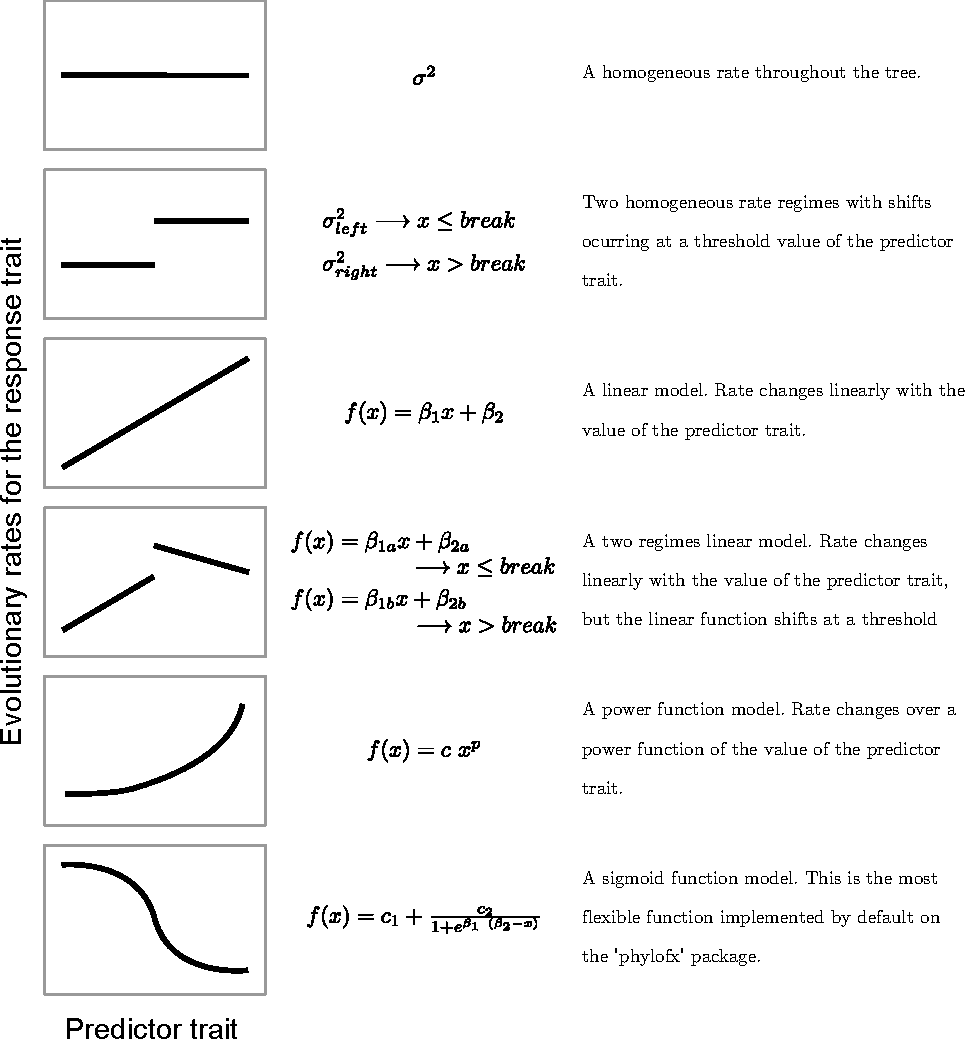
\includegraphics[scale=0.95]{Ch4_math_functions}
	\caption[List of mathematical functions implemented in the R package \texttt{phylofx}.]{List of mathematical functions implemented in the R package \texttt{phylofx}. Plots on the left show regression lines between the values of the predictor trait and the rates of evolution of the response trait ($\sigma^{2}_{response}$). Middle column shows the mathematical function(s) associated with each plot and right column provides a brief description of each function. These functions are easily selected from a menu when using the \texttt{phylofx}, however any mathematical function that associates trait predictor trait values to $\sigma^{2}_{response}$ can be implemented on \texttt{phylofx}.}
	\label{fig:bio_functions}
\end{figure}

\begin{figure}[hp]
	\centering
	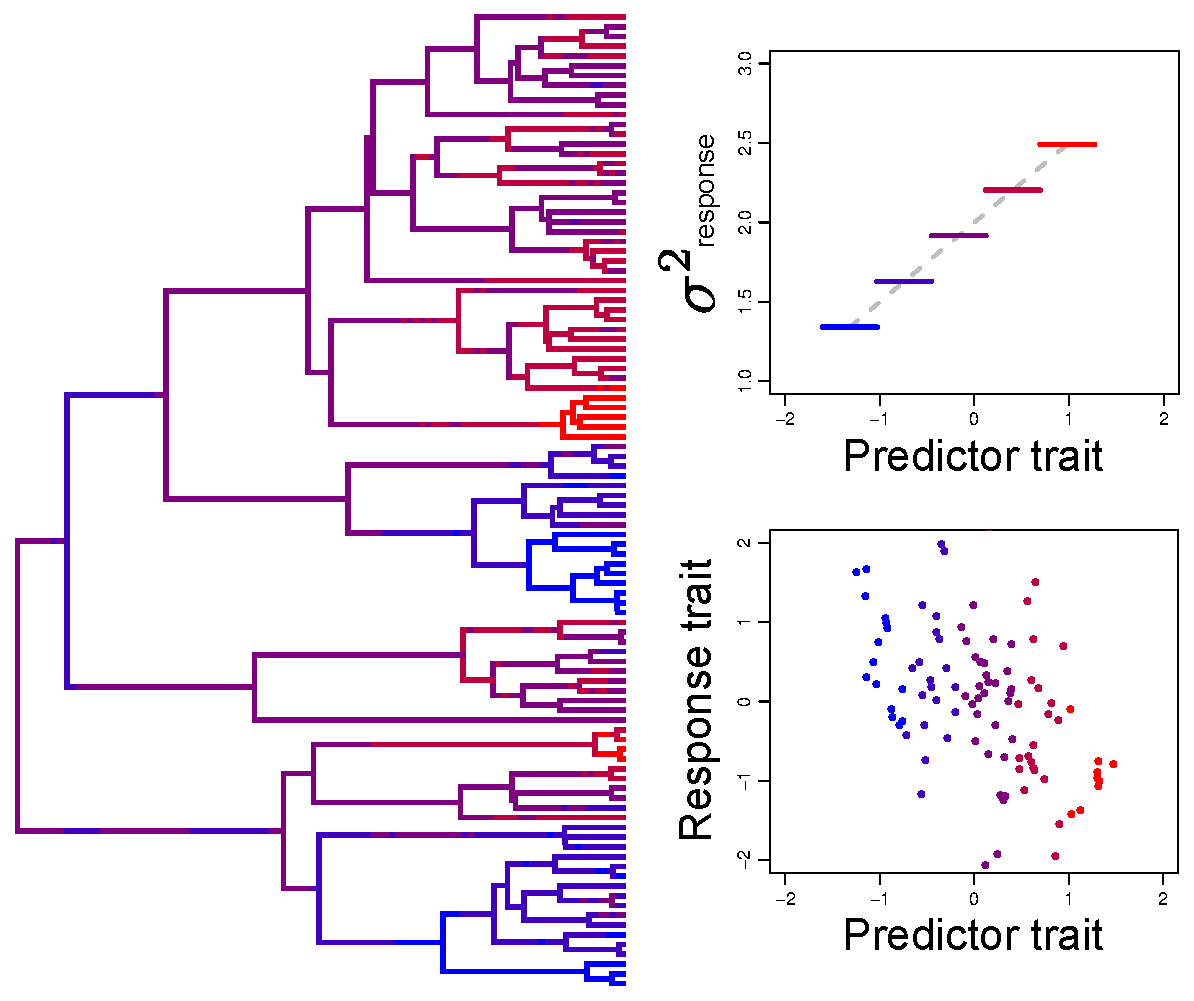
\includegraphics[scale=0.8]{Ch4_model_figure}
	\caption[Example of phylogeny showing changes in $\sigma^{2}$ for the response trait across the branches in function of the predictor trait values following a linear model with positive slope.]{Example of phylogeny showing changes in $\sigma^{2}$ for the response trait across the branches in function of the predictor trait values following a linear model with positive slope. Cold and warm colors represent slower and faster evolutionary rates, respectively. All colors match among plots. Each portion of a branch showed in the phylogenetic tree on the left is mapped to a value of $\sigma^{2}_{response}$ following the ancestral reconstructed value for the predictor trait. The relationship between the rate of evolution and the predictor trait value is shown on the upper right plot. The dashed gray line represents the linear function that generated the data (see main text for information on parameter values). Each horizontal line is one of the five rate categories ($\mathit{k}$) used to discretize the continuous gradient of rates. All predictor trait values on the extent of these horizontal lines are mapped to a respective $\sigma^{2}_{response}$ value. Bottom right plot show a scatter plot between the predictor and response trait values for the tips of the tree. See that there is no clear correlation between the trait values, since the association here is between the predictor trait values and the rates of trait evolution of the response trait.}
	\label{fig:model_example}
\end{figure}

\begin{figure}[hp]
	\centering
	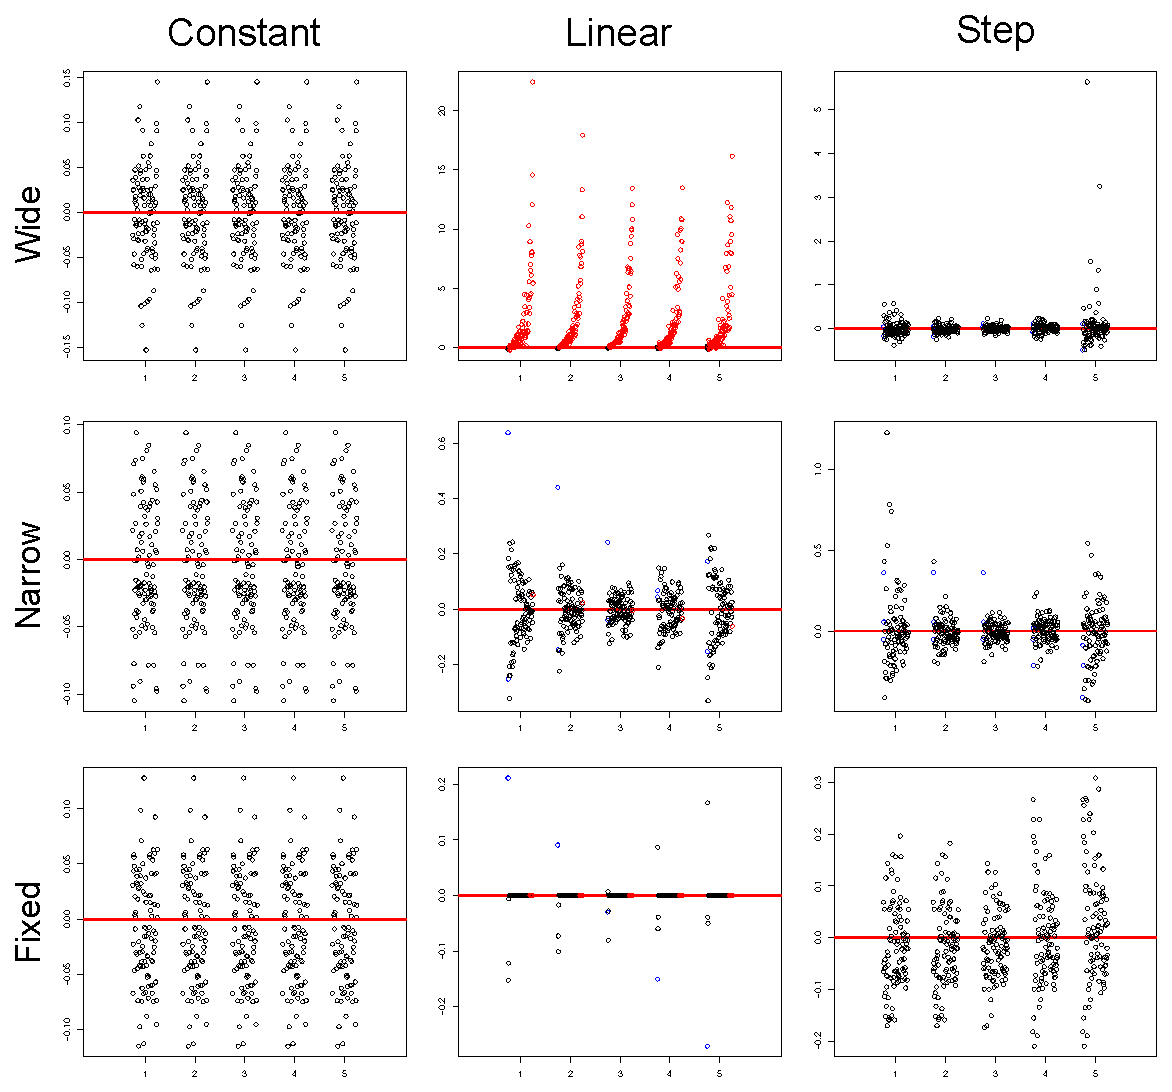
\includegraphics[scale=0.8]{Ch4_true_const_plots}
	\caption[Results from performance simulations using datasets generated with a constant evolutionary rate.]{Results from performance simulations using datasets generated with a constant evolutionary rate. Each plot shows the distance between the true value for the evolutionary rate and the estimated value for each of the 5 predictor trait categories used in the analyses. Columns show parameter estimates under different models and rows correspond to three search strategies. The x axes are the predictor trait categories from 1 to 5 while y axes show $\sigma^{2}_{response}$ associated with each category. The horizontal red line marks 0, which correspond to parameter estimates equal to the true value used to generate the data. The color of the points mark if the model is significantly better (threshold of 4 $\Delta$AIC units) than the model that generated the data (blue), worse than the generating model (red), or show no significant difference (black). Each point is the mean parameter estimate across stochastic mapped histories for each of the 100 simulations. Points were slightly dislocated horizontally for better visualization.}
	\label{fig:chart_const}
\end{figure}

\begin{figure}[hp]
	\centering
	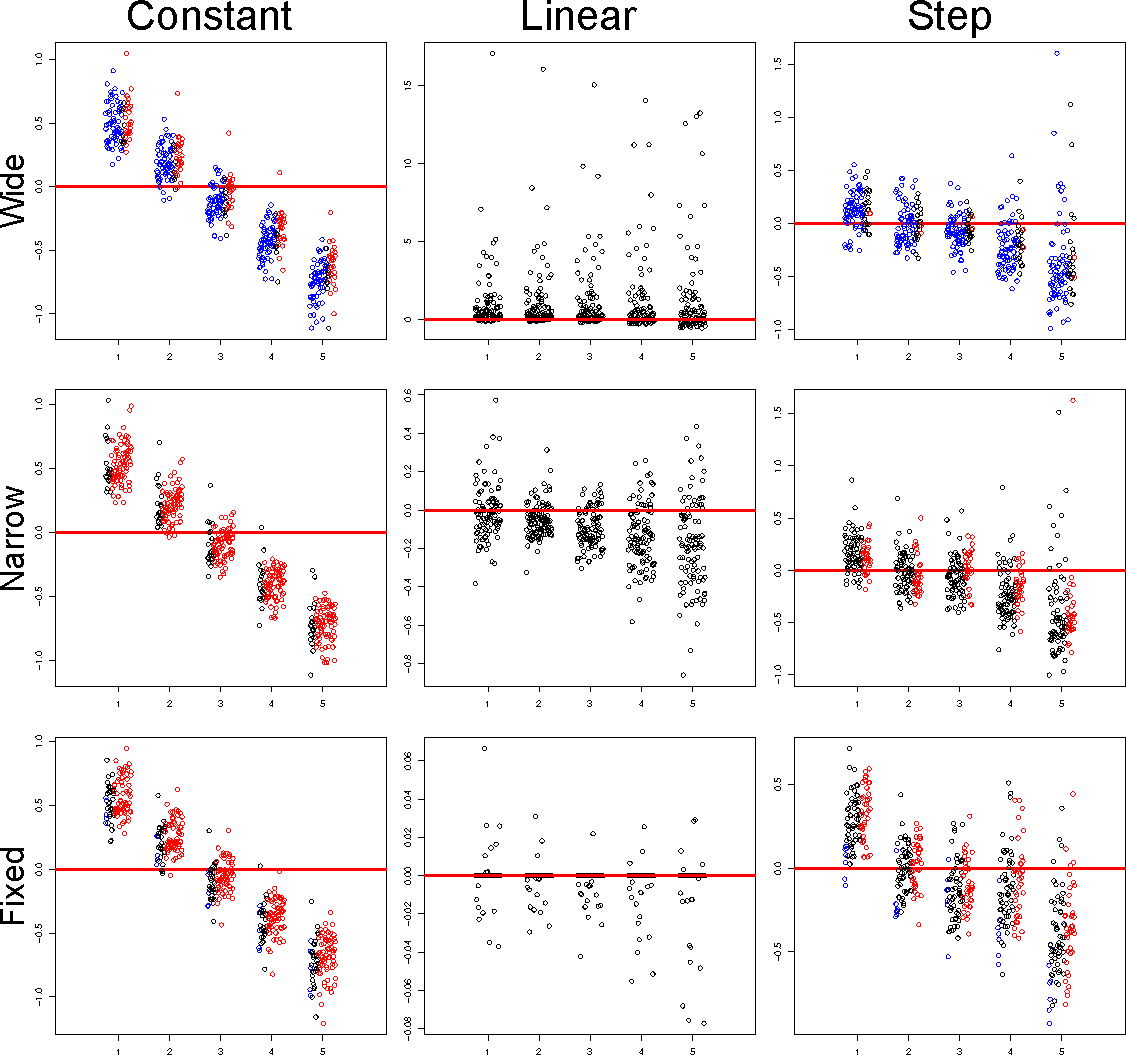
\includegraphics[scale=0.8]{Ch4_true_linear_plots}
	\caption[Results from performance simulations using datasets generated with a linear function between predictor trait values and rates of evolution of the response trait.]{Results from performance simulations using datasets generated with a linear function between predictor trait values and rates of evolution of the response trait. Each plot shows the distance between the true value for the evolutionary rate and the estimated value for each of the 5 predictor trait categories used in the analyses. Columns show parameter estimates under different models and rows correspond to three search strategies. The x axes are the predictor trait categories from 1 to 5, y axes show $\sigma^{2}$ associated with each category. The horizontal red line marks 0, which correspond to parameter estimates equal to the true value used to generate the data. The color of the points mark if the model is significantly better (threshold of 4 $\Delta$AIC units) than the model that generated the data (blue), worse than the generating model (red), or show no significant difference (black). Each point is the mean parameter estimate across stochastic mapped histories for each of the 100 simulations. Points were slightly dislocated horizontally for better visualization.}
	\label{fig:chart_linear}
\end{figure}

\begin{figure}[hp]
	\centering
	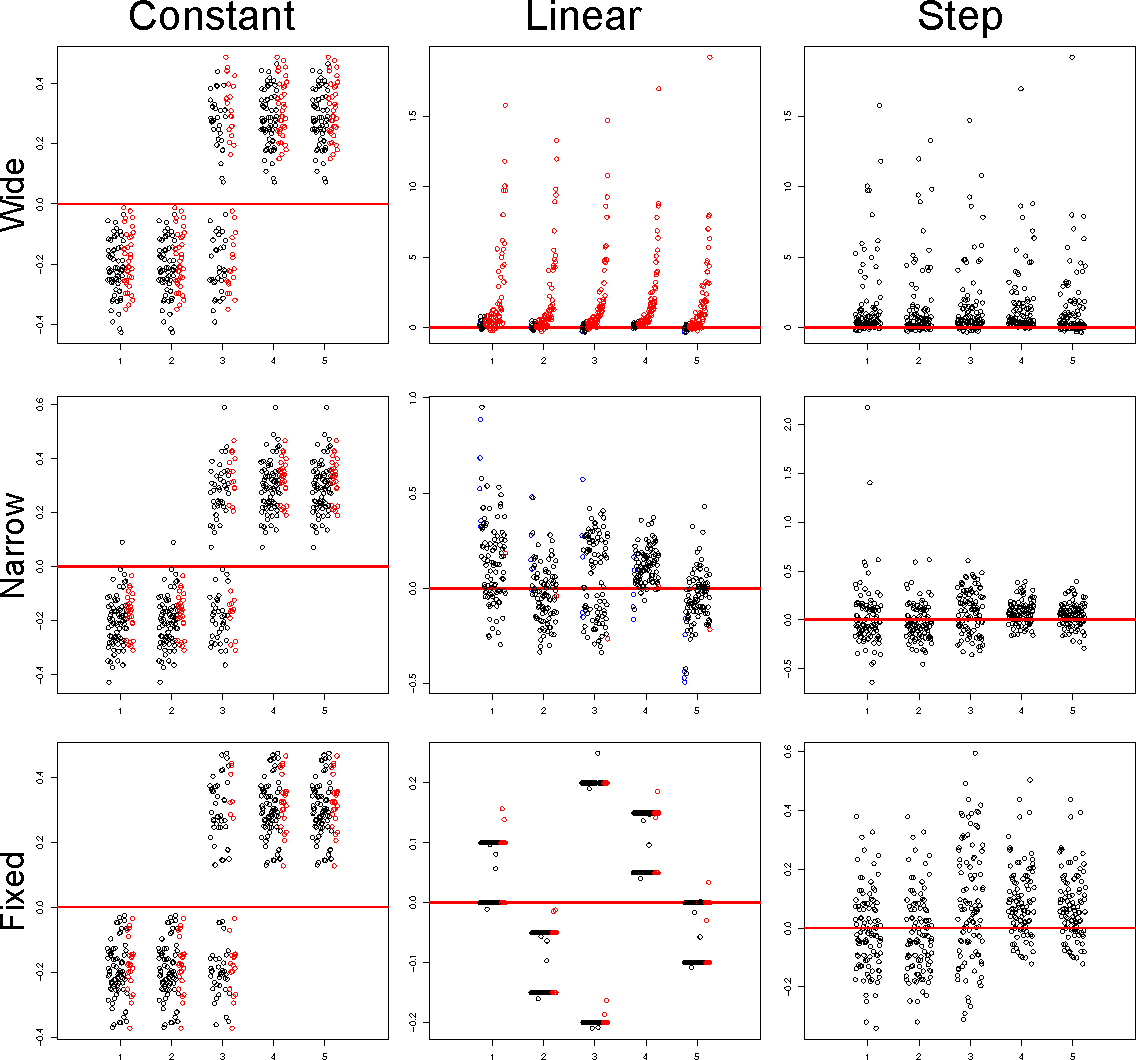
\includegraphics[scale=0.8]{Ch4_true_step_plots}
	\caption[Results from performance simulations using datasets generated with a step function between predictor trait values and rates of evolution of the response trait.]{Results from performance simulations using datasets generated with a step function between predictor trait values and rates of evolution of the response trait. Each plot shows the distance between the true value for the evolutionary rate and the estimated value for each of the 5 predictor trait categories used in the analyses. Columns show parameter estimates under different models and rows correspond to three search strategies. The x axes are the predictor trait categories from 1 to 5, y axes show $\sigma^{2}$ associated with each category. The horizontal red line marks 0, which correspond to parameter estimates equal to the true value used to generate the data. The color of the points mark if the model is significantly better (threshold of 4 $\Delta$AIC units) than the model that generated the data (blue), worse than the generating model (red), or show no significant difference (black). Each point is the mean parameter estimate across stochastic mapped histories for each of the 100 simulations. Points were slightly dislocated horizontally for better visualization.}
	\label{fig:chart_step}
\end{figure}

\begin{figure}[hp]
	\centering
	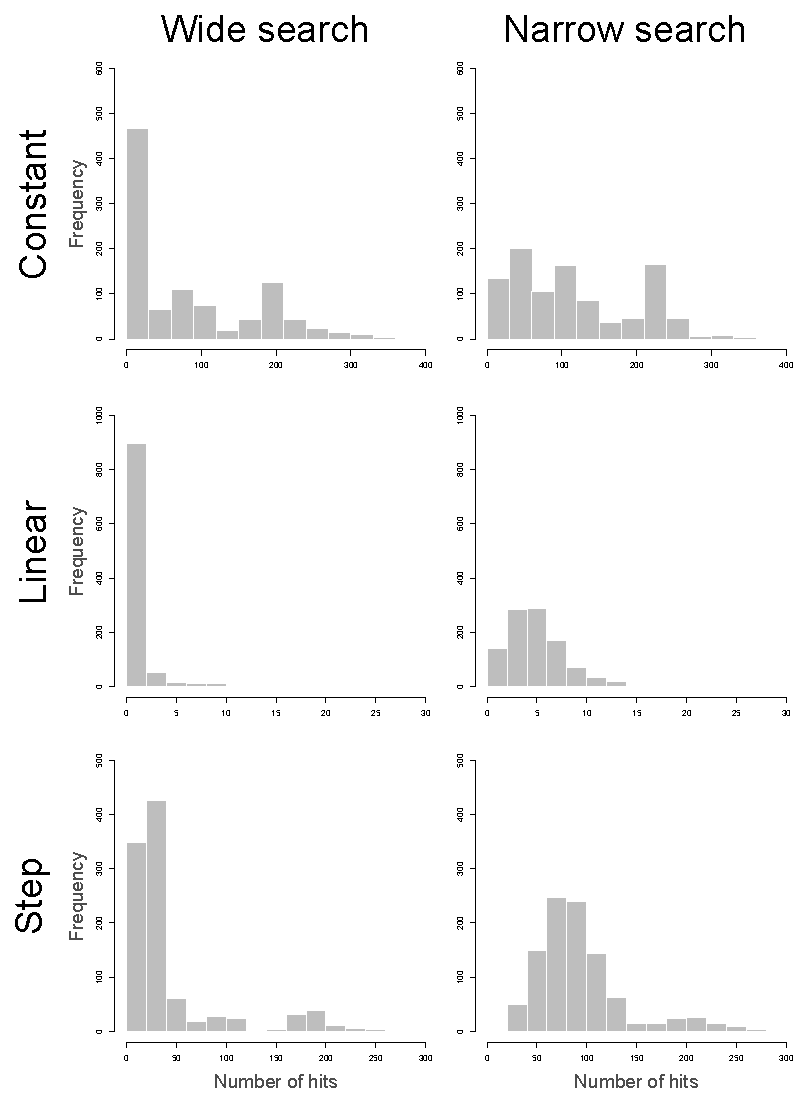
\includegraphics[scale=0.8]{Ch4_hist_hits_edited}
	\caption[Number of `hits' computed across each of the stochastic mapped histories for each simulation replicate and model.]{Number of `hits' computed across each of the stochastic mapped histories for each simulation replicate and model. Large number of `hits' means that multiple independent searches converged to the same log-likelihood score (with tolerance of 0.0001) and, as a result, same parameter values for the model. A total of 500 independent searches was conducted for each data set.}
	\label{fig:hist_hits}
\end{figure}

\begin{figure}[hp]
	\centering
	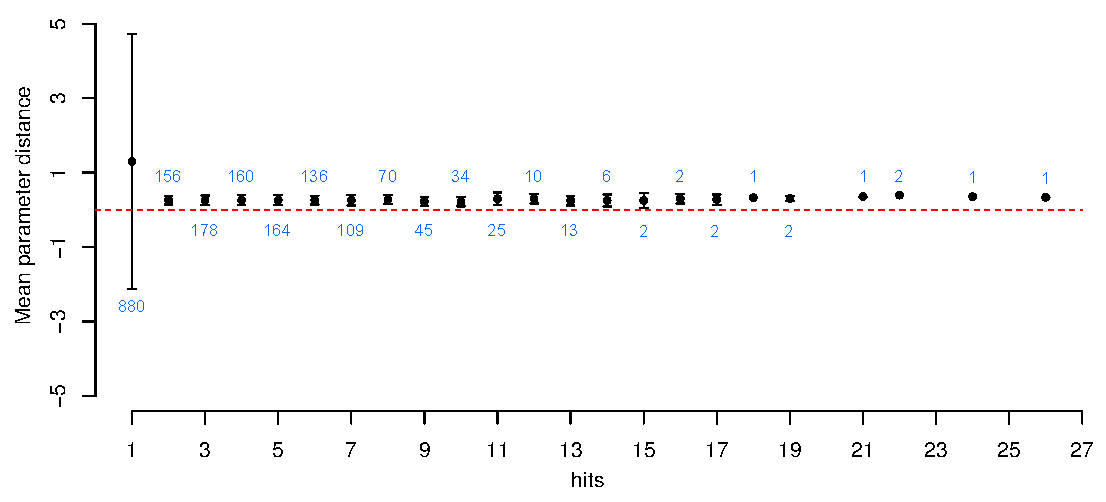
\includegraphics[scale=0.85]{Ch4_pardist_vs_hits}
	\caption[Relationship between the mean absolute distance of parameter estimates from the parameter values that generated the data and the number of `hits' after 500 independent searches.]{Relationship between the mean absolute distance of parameter estimates from the parameter values that generated the data and the number of `hits'. Plot show the results for 2000 datasets generated using the linear function and estimated using the same model. For each replicate we performed 500 independent searches for the best log-likelihood score starting from random points in the parameter space (using both the `wide' and `narrow' starting point strategies). Points show the mean absolute distance between the estimated and the true parameter values for each parameter of the model (i.e., slope and intercept). Bars around the points show standard deviations and sample size numbers are shown above or below each point. The dashed red line marks when estimated parameter values are identical to the parameter values that generated the data.}
	\label{fig:pardist}
\end{figure}